\documentclass[twocolumn,a4j]{jsarticle}
\renewcommand{\figurename}{fig.}
\renewcommand{\tablename}{Table }
\setlength{\topmargin}{-20.4cm}
\setlength{\oddsidemargin}{-10.4mm}
\setlength{\evensidemargin}{-10.4mm}
\setlength{\textwidth}{18cm}
\setlength{\textheight}{26cm}

\usepackage[top=15truemm,bottom=25truemm,left=20truemm,right=20truemm]{geometry}
\usepackage[latin1]{inputenc}
\usepackage{amsmath}
\usepackage{amsfonts}
\usepackage{amssymb}
\usepackage[dvipdfmx]{graphicx}
\usepackage{listings}
\usepackage{listings,jvlisting}
\usepackage{geometry}
\usepackage{framed}
\usepackage[T1]{fontenc}
\usepackage{textcomp}
\usepackage{graphics}

\lstset{
basicstyle={\ttfamily},
identifierstyle={\small},
commentstyle={\smallitshape},
keywordstyle={\small\bfseries},
ndkeywordstyle={\small},
stringstyle={\small\ttfamily},
frame={tb},
breaklines=true,
columns=[l]{fullflexible},
xrightmargin=0zw,
xleftmargin=3zw,
numberstyle={\scriptsize},
stepnumber=1,
numbersep=1zw,
lineskip=-0.5ex
}

\makeatletter
\def\@maketitle
{
\begin{center}
{\LARGE \@title \par}
\end{center}
\par\vskip 1.5em
}
\makeatother

\author{}
\title{資料収集について}
\date{}

\begin{document}
\maketitle
\section{\large 収集内容について}
\subsection{実験装置について}
先行研究において,以下のようなタイヤモデル及び地面板を設置した回流水槽を用いて実験を行っていた.\par
\begin{figure}[htbp]
    \begin{center}
        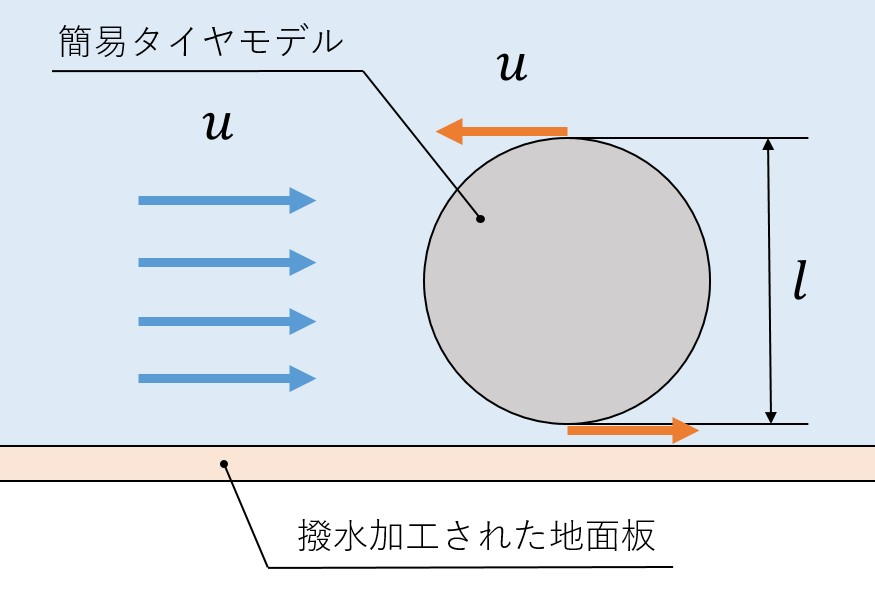
\includegraphics[width=80mm]{images/image_1.jpg}
        \caption{実験装置の概略図}
    \end{center}
\end{figure}
ここで,実験環境と現実環境における条件の差がどのように影響されるかについて考える.考えられる条件の相違点は以下の2点が挙げられる.
\begin{itemize}
    \item レイノルズ数の違いによる流れ場への影響
    \item 撥水性地面板の影響
\end{itemize}
\section{\large レイノルズ数}
\subsection{レイノルズ数とは}
レイノルズ数(以下$Re$)とは,「慣性力」と「粘性力」の比をとった無次元数を表す.
\begin{framed}
    \begin{eqnarray*}
        Re=\frac{\rho u l}{\mu}=\frac{u l}{\nu}
    \end{eqnarray*}
\end{framed}
\begin{itemize}
    \item $l$ : 代表長さ
    \item $u$ : 代表流速
    \item $\rho$ : 流体密度
    \item $\mu$ : 粘性係数
    \item $\nu$ : 動粘性係数
\end{itemize}
\par
分母が「粘性力」,分子が「慣性力」を表しており,
粘性力が支配的,すなわち$Re$が小さい場合,層流となる.
対して,慣性力が支配的,すなわち$Re$が大きい場合,流れは乱流となる.
\\
\textreferencemark 代表長さの選択については、\underline{どこでも良い!}\\
$Re$の比較を行う場合は、ひとつの代表長さに決める必要があるだけ!
\\
\subsection{実験環境,現実環境における$Re$}
先行研究より,実験環境及び現実環境における$Re$の値は以下のように示されている.
\begin{itemize}
    \item 実験環境 : $1.2 × 10^4$
    \item 現実環境 : $6 \sim 8 × 10^5$
\end{itemize}
\subsubsection{実験環境の$Re$について}
先行研究による実験環境における代表長さ及び代表速度は,以下のように記されている.
\begin{itemize}
    \item $l = 50\,[\mathrm{mm}]$
    \item $u = 250\,[\mathrm{mm/s}]$
\end{itemize}
また,実験環境を摂氏20度としたとき,水の密度$\rho$および,粘性係数$\mu$は,
\begin{itemize}
    \item $\rho = 998.20413\,[\mathrm{kg/m^3}]$
    \item $\mu = 0.0010017488\,[\mathrm{Pa\,s}]$
\end{itemize}
以上の値を用いて,$Re$を計算すると,
\begin{eqnarray}
    Re = 124555.76898\dots = 1.25 × 10^4
\end{eqnarray}
\subsubsection{現実環境の$Re$について}
同様に,$Re$を求める際のパラメータを以下のように定める.
\begin{itemize}
    \item $l = 600\,[\mathrm{mm}]$
    \item $u = 60\,[\mathrm{km/h}]$
    \item $\rho = 998.20413\,[\mathrm{kg/m^3}]$
    \item $\mu = 0.0010017488\,[\mathrm{Pa\,s}]$
\end{itemize}
なお,一般的な乗用車におけるタイヤサイズは,$500[\mathrm{mm}] \sim 700[\mathrm{mm}]$ 程度であったため,
ここでは,$600[\mathrm{mm}]$を採用している.
以上を用いて,$Re$を計算すると,
\begin{eqnarray}
    Re = 9964615.181\dots = 1.0 × 10^7
\end{eqnarray}
\subsection{$Re$の違いによる影響}



\end{document}